\chapter{Problem'atica}

Debido al crecimiento de Internet visto en el C'apitulo \ref{desarrolloWeb} y a los problemas que presenta el protocolo HTTP en su implementaci'on (visto en el C'apitulo \ref{protocolos}), se busca mejorar los tiempos de carga de los sitios web. 

%PONER PORQUE SE BUSCA MEJORAR LOS TIEMPOS DE RESPUESTA.

\section{T'ecnicas de optimizaci'on}

Es importante conocer d'onde es que el usuario pasa el tiempo esperando en la carga de un sitio web. Seg'un el estudio de Steve Souders en su libro \citep{highPerformanceWebSites}, el cliente tarda menos del 20\% para obtener el documento HTML, y el tiempo restante para recibir el resto de los componentes del sitio. Es importante enfocarse en el 80\%, 90\% restante, ya que el tiempo no se desperdicia en descargar el documento HTML ni en el procesamiento que realiza el servidor antes de enviarnos la petici'on. Esto se resume en la ''Regla de Oro de la Performance'' de dicho libro:

\begin{quote}

\textit{Solo el 10-20\% del tiempo de respuesta del usuario es consumido descargando el documento HTML. El otro 80-90\% se consume descargando todos los componentes de la p'agina.}

\end{quote}

Plantea 14 reglas para la optimizaci'on de los sitios que se describen a continuaci'on.

\begin{enumerate}

\item \textbf{Minimizar la cantidad de peticiones.}

La idea b'asica es eliminar las peticiones al servidor, esto se hace utilizando varias t'ecnicas enumeradas a continuaci'on.

	\begin{enumerate}
	\item Mapa de Im'agenes - Permite asociar m'ultiples 'areas en una imagen para que se puedan cliquear y realizar cierta acci'on (el ejemplo m'as b'asico es el de navegar un hiperv'inculo). En vez de utilizar m'ultiples im'agenes para realizar un men'u por ejemplo, se utilizar'ia una sola mapeada. De esta manera se ahorran las peticiones de las im'agenes por 1 sola petici'on.
	\item CSS Sprites - Permite combinar v'arias im'agenes en una sola, luego en el sitio, se define que parte de la imagen combinada desea mostrarse. Por ejemplo, en el sitio de Google cuando se realiza una b'usqueda, se utiliza el Sprite que se ve en la Figura \ref{css_sprites}.
		\begin{figure}[htbp]
		\begin{center}
			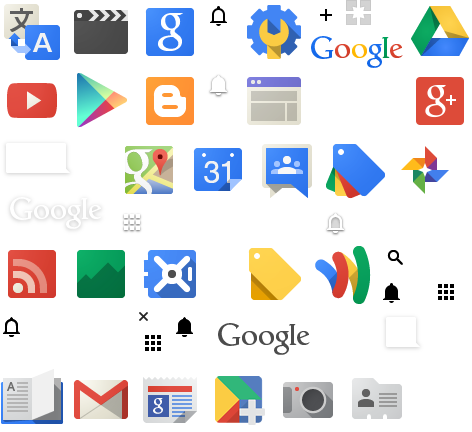
\includegraphics[width=150px]{img/css_sprites}
			\caption{\small Sprite del sitio www.google.com}
		\end{center}
		\label{css_sprites}
		\end{figure}

	A simple vista se ven 44 im'agenes combinadas. La utilizaci'on de este Sprite reducir'ia todas estas peticiones a 1 sola.
	\item Im'agenes Inline - Se pueden incluir im'agenes en un sitio web sin necesidad de realizar una petici'on al servidor definiendolas con el esquema \textit{data:} \ref{rfcData} dentro del c'odigo HTML de la p'agina.
	\item Combinar Scripts y Hojas de Estilo - Como la mayor'ia de los sitios actuales utilizan Javascript y CSS, es preferible que los Scripts se combinen en uno solo al igual que las Hojas de Estilo. En el caso de tener varios archivos, el navegador va a generar una petici'on por cada uno de ellos de no tenerlo almacenado en una copia local.
	\end{enumerate}
\item \textbf{Utilizar un CDN}

La proximidad del cliente al servidor web tiene un impacto en el tiempo de respuesta de las peticiones. No es lo mismo solicitar un recurso localizado China estando en Argentina que uno ubicado dentro del mismo pa'is. Por ende, si los contenidos est'an cerca\footnote{En t'erminos de distancia f'isica.} el tiempo de respuesta es menor. Debido a que solo el 10-20\% del tiempo de respuesta se dedica al HTML (visto al inicio de este cap'itulo), si el resto de los recursos del sitio se encuentran cerca del cliente, se mejorar'ian los tiempos de respuesta. Para esto es necesario dispersar estos recursos geogr'aficamente.

Un CDN\footnote{Content Delivery Networks} es una red de distribuci'on de contenidos. Son servidores dispersados geogr'aficamente que ofrecen r'eplicas de los recursos de un sitio particular para brindarlos al cliente desde el m'as cercano a su locaci'on.

Utilizar el servicio que brinda un CDN mejora los tiempos de respuesta de los usuarios.
\item \textbf{A'nadir Headers para Cach'es}

Cuando un usuario visita el sitio por primera vez, realiza tantas peticiones HTTP como recursos tenga la p'agina. Utilizando Headers Expires o Cache-Control\footnote{Desde HTTP 1.1} (Cap'itulo \ref{protocolos}, Secci'on \ref{headers}) se puede hacer que los recursos puedan ser almacenados en Cach'es (Cap'itulo \ref{cache}). Esto disminuye la cantidad de peticiones en una posterior visita a la p'agina del mismo usuario.

La performance del tiempo de respuesta del sitio mejora seg'un la cantidad de ''Hits''\footnote{Necesidad de solicitar un recurso que ya tengo almacenado en la Cach'e} que el usuario tenga de los componentes del sitio.
\item \textbf{Comprimir los componentes (Gzip)}

Se puede reducir el tiempo de respuesta, disminuyendo el tama'no de la respuesta HTTP. Esto se puede realizar comprimiendo el recurso que se est'a solicitando. La reducci'on del tiempo es mayor en ambientes en donde el ancho de banda es bajo. El formato \textit{Gzip}\footnote{http://www.gzip.org/} \citep{rfcGzip} es el m'as popular y el m'as efectivo, el otro formato que se usa con menos frecuencia es \textit{deflate} \citep{rfcDeflate}.

El usuario tiene que enviar en la petici'on un Header \textit{Accept-Encoding} indicando los m'etodos aceptados. Cuando el servidor recibe este Header, puede comprimir el recurso utilizando alguno de los m'etodos indicados por el usuario. Este devuelve la respuesta con un Header \textit{Content-Encoding} indicando el tipo de compresi'on utilizado en el recurso que se est'a enviando.

Los tipos de archivos que se deber'ian comprimir son aquellos de texto, tales como HTML, Scripts, CSS, etc. Aquellos formatos que ya se encuentran comprimidos como las im'agenes o los archivos PDF no deber'ian comprimirse ya que se desperdicia tiempo de CPU del servidor\footnote{Para realizar la compresi'on.} y adem'as puede incluso incrementar el tama'no del archivo.

\item \textbf{CSS en el Head del HTML}
\item \textbf{Scripts en la parte inferior del HTML}
\item \textbf{Evitar expresiones en CSS}
\item \textbf{Utilizar JavaScript y CSS de manera externa (no inline)}
\item \textbf{Reducir las b'usquedas de DNS (keep-alive y pocos dominios)}
\item \textbf{Minificar el JavaScript}
\item \textbf{Evitar redirecciones}
\item \textbf{Remover Scripts duplicados}
\item \textbf{Configurar Etags}
\item \textbf{Hacer que Ajax pueda ser Cacheado (BUSCAR OTRA PALABRA)}

\end{enumerate}